\documentclass[9pt,twocolumn,twoside]{styles/osajnl}
\usepackage{fancyvrb}
\usepackage[colorinlistoftodos,prependcaption,textsize=normal]{todonotes}
\newcommand{\TODO}[2][]{\todo[color=red!10,inline,#1]{#2}}
\newcommand{\GE}{\TODO{Grammar}}
\newcommand{\SE}{\TODO{Spelling}}
\newcommand{\TE}{\TODO{Term}}
\newcommand{\CE}{\TODO{Citation}}
\journal{i524} 

\title{CUBRID RDBMS}

\author[1]{Abhijit Thakre}

\affil[1]{School of Informatics and Computing, Bloomington, IN 47408, U.S.A.}
\affil[2]{Mechanical Engineer,Nagpur University, 2003}

\affil[*]{Corresponding authors: abhijit.thakre@gmail.com}

\dates{project-000, \today}

\ociscodes{Cloud, I524}

% replace this with your url in github/gitlab
\doi{\url{https://github.com/cloudmesh/classes/blob/master/docs/source/format/report/report.pdf}}

\begin{abstract}

With advanced techniques of data mining and analysis, bigdata
processing has become a key in today’s world.  Many of the bigdata
processing uses NOSQL data for storing. However in order to avail the
ACID behavior of database, the focus is again back to the RDBMS
databases. This paper focuses on one the similar ORDBMS CUBRID. It
also highlight the architecture of CUBRID with it key component and
features provided.
  
\end{abstract}


\setboolean{displaycopyright}{true}

\begin{document}

\maketitle

\TODO{This review document is provided for you to achieve your
  best. We have listed a number of obvious opportunities for
  improvement. When improving it, please keep this copy untouched and
  instead focus on improving report.tex. The review does not include
  all possible improvement suggestions and if you sea comment you may
  want to check if this comment applies elsewhere in the document.}

\section{Introduction}

CUBRID is open source RDBMS with object support developed by Navel
corporation. Developed in C language CUBRID provides key features like
scalability, high availability, higher performance, online and
incremental backups. CUBRID is distributed under GNU general public
license for the database server engine and BCD license for API and
client tool.

\section{Architecture}

CUBRID has distinguished 3 layer architecture.  It consists of
Database server, connection broker and application layer.

\subsection{Database Server}

Â\SE It is the core component of the CUBRID Database Management
System. The main function for the database server are as below
\begin{itemize}
\item Saving and managing the data.
\item Processing of the queries from user.
\item Providing smooth functioning for multiple users.
\end{itemize}
\subsection{Broker}

It acts as middleware between the Database Server and GUI application
to provide seamless experience.
It provides functions
\begin{itemize}
\item Connection pooling.
\item Monitoring.
\item Log tracing and analysis.
\end{itemize}
\subsection{CUBRID Manager}
\TODO{the above two subsections appear like a slide page. try to use less bullet points}
 It is a GUI tool that manages database and broker. It also provides
the Query Editor for executing queries on database for users.

\section{Overall Architecture}
\TODO{1. you usually don't have an "overall architechture" after an "architechture" 2. name your figure}

\begin{figure}[htbp]
\centering
\fbox{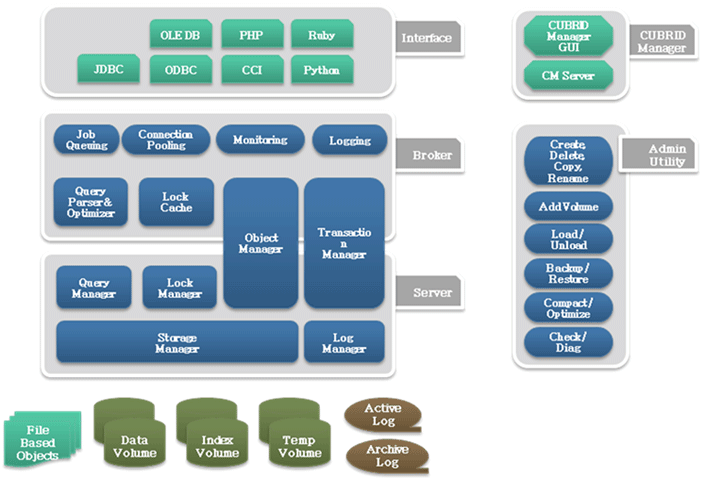
\includegraphics[width=\linewidth]{images/cubrid_architecture}}
\caption{\cite{www-cubrid.org}}
\label{Reference:false-color}
\end{figure}

\newpage

\section{Description}

Database server and the broker work in co-ordination with each other
as server and client respectively. The can be deployed on the
different or same machine. The broker takes care of the queries from
the users, it process it to the optimum level. On optimization it
creates a query plan tree and sends the request to the server. The
response from the server is via cursor navigation which is further
returned to the user.

The client caches object instances from the
database to its memory to provide fast access to data by using the
query execution results or directly by users/applications. In
addition, it caches locks as well as objects from the server for
concurrency control. The execution of triggers or methods specified by
users or applications is also performed in the client module.

References: \cite{www-cubrid.org}
\newpage

\TODO{please fix the "References" and do not split the page in the middle}

\section{Module Configuration}

The CUBRID client and server modules consist of the following components:

\begin{itemize}
\item Transaction Management Component.
\item Server Storage Management Component.
\item Client Storage Management Component.
\item Object Management Component.
\item Client-Server Communications.
\item Thread Management.
\item Query Processing.
\end{itemize}

\section{Authentication in CUBRID}


CUBRID provides two levels of authentication.

User needs to enter credentials to login to the Host Server. On first
login user need to set the admin credentials.

User needs to login to each database in the host server to access the
individual database.
Reference : \cite{www-authentication}


\section{Key Features}

\subsection{High Availability and Scalability}

CUBRID uses heartbeat technology to
provide automated accurate fail-over and fail-back features which
makes the database continuously available. The server is available
during the upgrades, replacement or even during the maintenance phase.

\subsection{Database Sharding}

CUBRID 8.4.3 provides free sharding feature where data can be divided
on multiple instance.  In addition to unlimited sharding it also
provides the features like connection pooling and load balancing to
all the shards.

\subsection{Performance}

CUBRID provides high performance to the users with feature like query
caching, optimized algorithm for indexing, fast object access.

Function based indexing, filtering indexing and index skip scan
provides various features to user for increasing the performance

\subsection{Reliability}

CUBRID is highly reliable with features like online incremental backup
and restore.  It provides the access restriction based on userip and
databaseid.

\subsection{Language Support}
It provides 90 percent support to sql language support. 


\section{CUBRID SHARD}

CUBRID shard is sharding is RDBMS specially targeted to address the
problem on processing bigdata. CUBRID shard distributes the user data
on multiple server to store it. So for fetching the data specific to
user it needs to pass key information about the shard in the
query. Parsing the query and finding the shard both things are taken
care by the broker and does not needs the additional layer. This helps
in increasing the performance for big data. 

\newpage

% Bibliography

\bibliography{references}
 
\section*{Author Biographies}
\begingroup
\setlength\intextsep{0pt}
\begin{minipage}[t][3.2cm][t]{1.0\columnwidth} % Adjust height [3.2cm] as required for separation of bio photos.
  \begin{wrapfigure}{L}{0.25\columnwidth}
    
\includegraphics[width=0.25\columnwidth]{images/john_smith.eps}
  \end{wrapfigure}
  \noindent
  {\bfseries Abhijit Thakre} received his BE (Mechanical) in 2003 from
  The University of Nagpur.
\end{minipage}
\endgroup


\appendix

\end{document}
